[4~v\textsuperscript{o}] causas, cur corpora majora longius projiciantur. Cur pendula\protect\index{Sachverzeichnis}{pendulum} et alia oscillantia cessent, cur corpus majus difficilius impellatur quam minus, etiam quando pondere caret, ut si in aqua bene libratum intelligatur. Et tunc experiundum est, discrimen ne notabile inter plumbum\protect\index{Sachverzeichnis}{plumbum}, et aliud corpus minus solidum, quod tamen solido circummunitum est; idemque circiter volumen occupat cum priore. Posset dici adhuc intra aquam esse resistentiam\protect\index{Sachverzeichnis}{resistentia} quandam in ipso cavo corporis, materiae aethereae\protect\index{Sachverzeichnis}{materia aetheria} cuncta pervadentis. Sed experimentum hoc plurimum lucis afferet. Pone corpus ejusmodi bene libratum exiguo arcu\protect\index{Sachverzeichnis}{arcus} horizontaliter explodi, et aliud similiter; videndum, an differentia in projectu. Dices \edtext{observatum est}{\lemma{observatum est}\Cfootnote{\cite{00050}\cite{00048}G. \textsc{Galilei}, \textit{Discorsi}, Leiden 1638, S. 76 (\textit{GO} VIII, S. 119f.)}} \edtext{si pila plumbea}{\lemma{si}\Bfootnote{\textit{(1)}\ globo \textit{(2)}\ pila \textit{(a)}\ aenea \textit{(b)}\ plumbea \textit{L}}} aut lignea ex summo tecto \edtext{simul}{\lemma{}\Bfootnote{simul \textit{erg.} \textit{L}}} demittantur, discrimen temporis quo terram attingant, vix ac ne vix quidem sensibile esse. Ita est fateor, sed hoc inde evenit, quod initium descensus lentum, cui parum obsistit aer aetherve\protect\index{Sachverzeichnis}{aether}, crescitque sane sed nondum satis in spatio \edtext{[non]}{\lemma{non}\Bfootnote{\textit{erg. Hrsg.}}} satis magno, ita ut \edtext{ultimus impetus lapidis descendentis}{\lemma{ultimus}\Bfootnote{\textit{(1)}\ ejus impetus \textit{(2)}\ impetus lapidis descendentis \textit{L}}}, non sit \edtext{forte}{\lemma{}\Bfootnote{forte \textit{erg.} \textit{L}}} major ejusdem primo impetu\protect\index{Sachverzeichnis}{impetus} a manu \edtext{projecti. Sed et}{\lemma{projecti.}\Bfootnote{\textit{(1)}\ Et \textit{(2)}\ Sed et \textit{L}}} quod ad celeritatem\protect\index{Sachverzeichnis}{celeritas} attinet, arbitror pilam\protect\index{Sachverzeichnis}{pila} plumbeam ligneamque arcu\protect\index{Sachverzeichnis}{arcus} projectas non usque adeo celeritate\protect\index{Sachverzeichnis}{celeritas} differre. \edtext{Sed differunt plurimum ictu quem inferent}{\lemma{Sed}\Bfootnote{\textit{(1)}\ impetu\protect\index{Sachverzeichnis}{impetus} differunt plurimum, quem in \textit{(2)}\ impetu\protect\index{Sachverzeichnis}{impetus} differunt plurimum, ictuque\protect\index{Sachverzeichnis}{ictus} \textit{(3)}\ differunt [...] inferent, \textit{L}}}, quemadmodum pila\protect\index{Sachverzeichnis}{pila} plumbea ligneaque; \edtext{quia pila\protect\index{Sachverzeichnis}{pila} plumbea}{\lemma{quia pila}\Bfootnote{\textit{(1)}\ lignea \textit{(2)}\ plumbea \textit{L}}} reapse pro majore haberi debet. Corpus autem agit non tantum celeritate\protect\index{Sachverzeichnis}{celeritas} sed et magnitudine. Perinde, ut trabs\protect\index{Sachverzeichnis}{trabs} a flumine acta, si major est, fortius agit, quia pars ejus quaelibet separatim a flumine impellitur, tenduntque omnes in idem ob connexionem; ut una impingente tota impingere videatur in pontem. Eodem modo quod flumen trabi id impetus\protect\index{Sachverzeichnis}{impetus} impressus, pilae\protect\index{Sachverzeichnis}{pila}, qui in quamlibet ejus partem egit, seu ei conatum\protect\index{Sachverzeichnis}{conatus} dedit. \edtext{Experiundum, si}{\lemma{Experiundum,}\Bfootnote{\textit{(1)}\ an \textit{(2)}\ si \textit{L}}} arcus\protect\index{Sachverzeichnis}{arcus} idem eodem modo tensus nunc pilam\protect\index{Sachverzeichnis}{pila} plumbeam majorem nunc minorem\textso{ in plano }\edtext{claritatis causa}{\lemma{claritatis causa}\Bfootnote{\textit{erg. L}}}\textso{ horizontali }projiciat, quae futura differentia, ratione celeritatis\protect\index{Sachverzeichnis}{celeritas} motus, et ratione ictus\protect\index{Sachverzeichnis}{ictus} quem dat. Haec in tabula marmorea \edtext{vel lignea}{\lemma{}\Bfootnote{vel lignea \textit{erg.} \textit{L}}}, arcu, adhibitis majoribus pilis, ne longius justo projiciat, et sub finem posita re mobili, cui pondus appensum\textso{ ex aqua }elevandum ita ut elevatum rursus intrare nisi nostro permissu nequeat, et ut tempus notetur, adhibendum pendulum vibrans saepissime, et cum incipit, finitque impinget in quaedam,\textso{ quae in pendulo}\protect\index{Sachverzeichnis}{pendulum}\textso{ notabunt.} Videndum quid fiat si arcus\protect\index{Sachverzeichnis}{arcus} duas simul pilas\protect\index{Sachverzeichnis}{pila} majorem minoremque projiciat, nunc ejusdem materiae nunc diversarum. Loco arcus\protect\index{Sachverzeichnis}{arcus} tensi adhiberi potest pondus cadens ex certa altitudine, et cadendo filum adducens, quod chordam agere facit, qualis est arcus\protect\index{Sachverzeichnis}{arcus}: et ita in tabula satis lata plura experimenta ejusmodi simul fieri possunt rectiusque discerni tempus.
\pend

\pstart
     \begin{wrapfigure}[13]{l}{0.23\textwidth}                    
    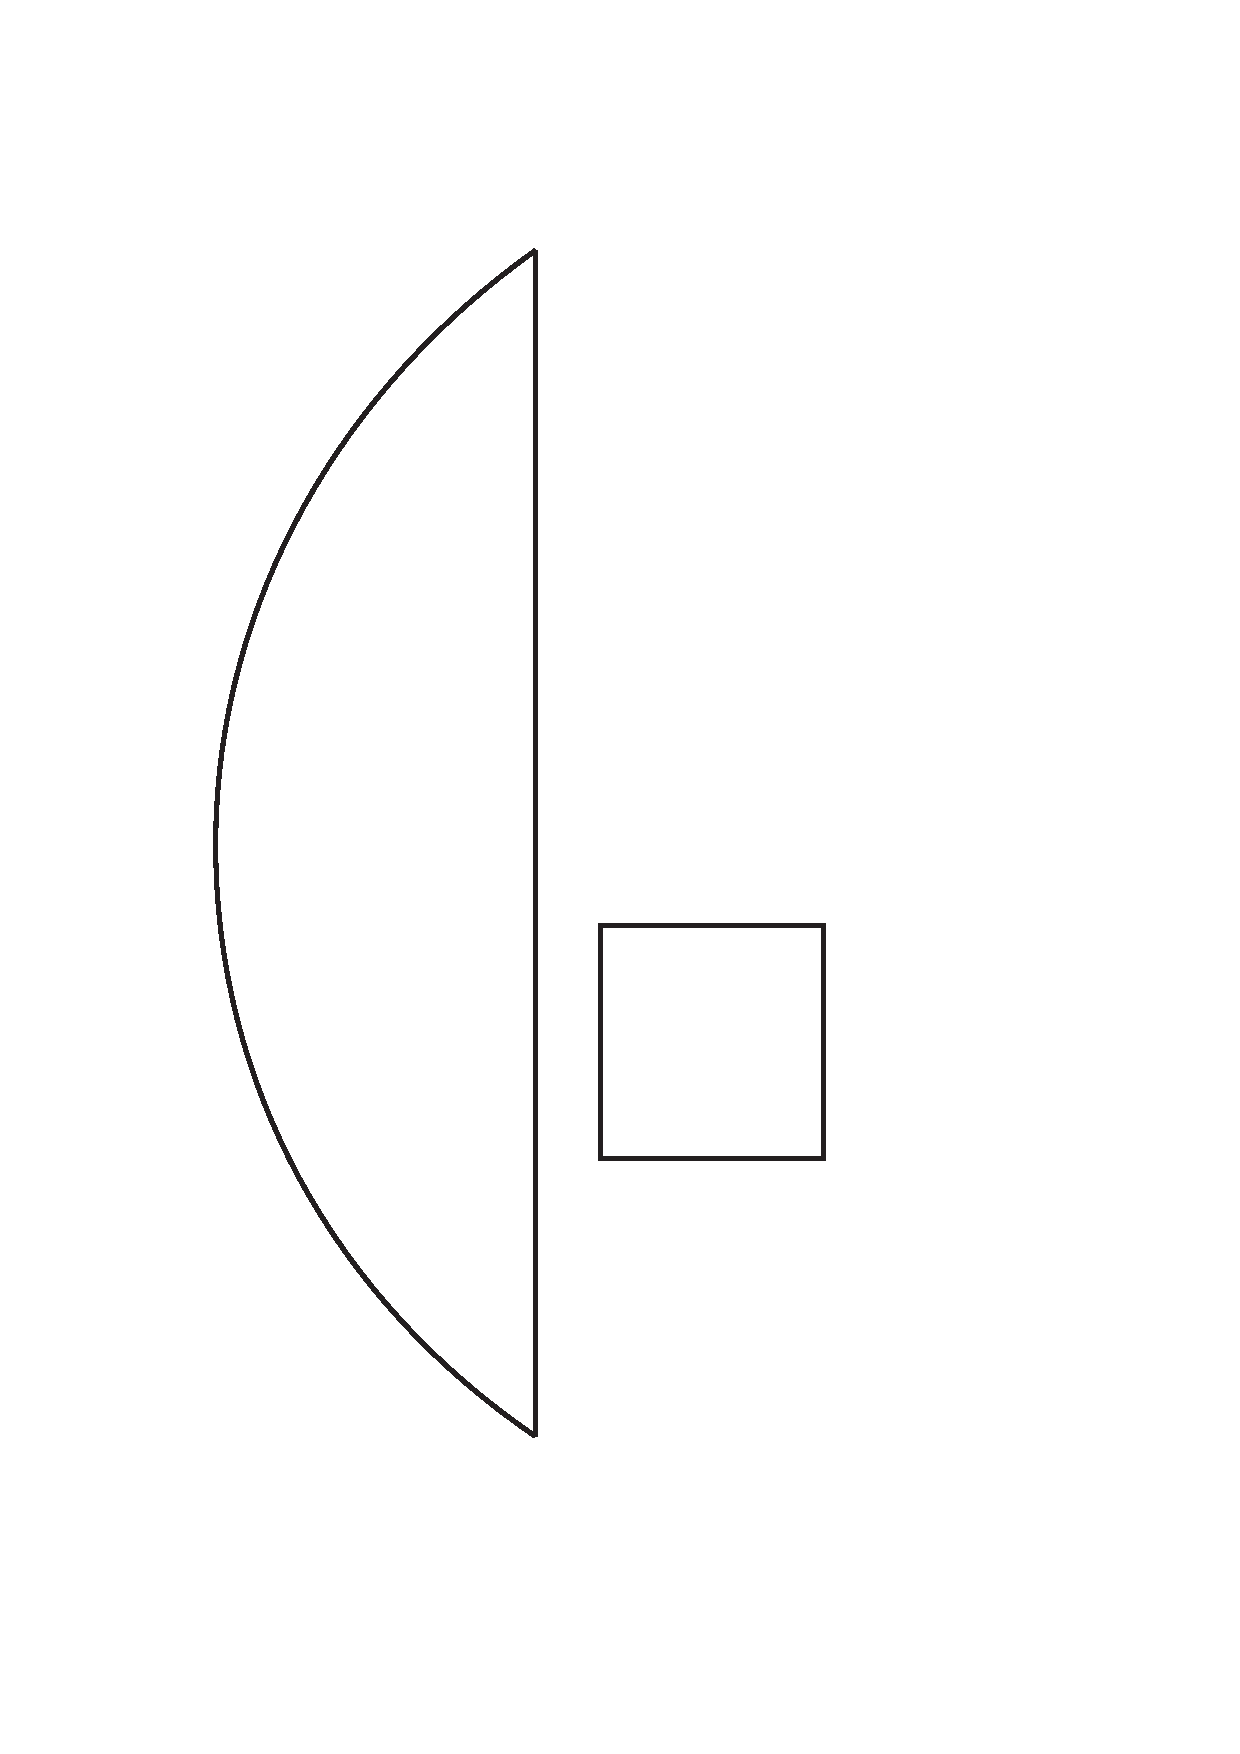
\includegraphics[trim = 36mm 48mm 60mm 42.5mm, clip,width=0.2\textwidth]{images/lh03705_004v-d1.pdf}
     % \caption{Bildbeschreibung}
 \noindent \centering [\textit{Fig. 2}] 
     \end{wrapfigure}
Si \edtext{ex arcu}{\lemma{ex}\Bfootnote{\textit{(1)}\ sclopeto \textit{(2)}\ arcu \textit{L}}} \edtext{emittatur pila\protect\index{Sachverzeichnis}{pila} proportionata,}{\lemma{emittatur pila}\Bfootnote{\textit{(1)}\ magna \textit{(2)}\ proportionata, \textit{L}}} et pila\protect\index{Sachverzeichnis}{pila} valde parva, quaestio est, an tantum impetus\protect\index{Sachverzeichnis}{impetus} sit in parva, quantum fuisset in \edtext{proportionata. Sane non est considerandum}{\lemma{proportionata.}\Bfootnote{\textit{(1)}\ Item \textit{(2)}\ Con \textit{(3)}\ Sane [...] considerandum \textit{L}}} quaenam pila\protect\index{Sachverzeichnis}{pila} sit proportionata, et cur Arcus\protect\index{Sachverzeichnis}{arcus} parvae isti pilae\protect\index{Sachverzeichnis}{pila} non tantum ictus\protect\index{Sachverzeichnis}{ictus} imprimet quantum magnae? Cur ita? An quia non imprimitur ictus, nisi quantum resistitur? Pila\protect\index{Sachverzeichnis}{pila} autem ista exigua non resistit. Et sane resistentiam videtur plurimum ad rem pertinere? Sed cur ita? Experiendum an res% \pend